\documentclass[11pt,a4paper]{report}
\usepackage[portuguese]{babel}
\usepackage[utf8]{inputenc}
\usepackage{graphicx}
\usepackage{url}
\usepackage{enumerate}
\usepackage{color}
\usepackage{xcolor}
\usepackage{multirow}
\usepackage{array}
\usepackage[pdftex]{hyperref}
\usepackage{listings}
\usepackage{xspace}
\usepackage{minted}
\usepackage{appendix}
\usepackage{amsmath}
\usepackage{titlesec}
\usepackage{hyperref}
\usemintedstyle{autumn}

\makeatletter
\newcommand\subsubsubsection{\@startsection{paragraph}{4}{\z@}{-2.5ex\@plus -1ex \@minus -.25ex}{1.25ex \@plus .25ex}{\normalfont\normalsize\bfseries}}
\newcommand\subsubsubsubsection{\@startsection{subparagraph}{5}{\z@}{-2.5ex\@plus -1ex \@minus -.25ex}{1.25ex \@plus .25ex}{\normalfont\normalsize\bfseries}}
\makeatother

\setcounter{secnumdepth}{4}
\setcounter{tocdepth}{4}

\definecolor{mls_orange}{HTML}{ab5400}

\parindent=0pt
\parskip=2pt

\setlength{\oddsidemargin}{-1cm}
\setlength{\textwidth}{18cm}
\setlength{\headsep}{-1cm}
\setlength{\textheight}{23cm}

\def\super#1{{\em Supervisor: #1}\\ }
\def\area#1{{\em \'{A}rea: #1}\\[0.2cm]}

\title{Processamento de Linguagens\\
       \textbf{Trabalho Prático}\\ Relatório de Desenvolvimento}

\author{João Paulo Machado Abreu\\ a91755
        \and Ricardo Cardoso Sousa\\ a96141
        \and Rui Pedro Guise da Silva\\ a97133}

\date{28 de maio de 2023}

\begin{document}
\maketitle

\begin{abstract}
\paragraph*{}
Este relatório aborda o desenvolvimento de uma extensão funcional, \textbf{\textit{FPY}}, para a linguagem de programação \textit{Python}, com recurso à ferramenta de análise \textit{ply}.
\end{abstract}

\tableofcontents

\chapter{Introdução} \label{chap:intro}
\paragraph*{}
A programação funcional é um paradigma de programação que se foca no uso de funções puras, dados imutáveis e funções de ordem superior. Linguagens de paradigma imperativo e orientado a objetos, como \textit{Python}, têm adotado alguns princípios provenientes deste paradigma de computação mas são ainda bastante limitadas comparativamente ao que é possível fazer numa linguagem puramente funcional. Por este motivo, decidimos aceitar um dos 8 desafios propostos no âmbito do trabalho prático da unidade curricular de \textit{Processamento de Linguagens} e desenvolver uma extensão funcional para \textit{Python}, com o objetivo de simplificar a escrita de funções em \textit{Python}, utilizando o paradigma funcional na escrita das mesmas e ainda implementar algumas funcionalidades inexistentes em \textit{Python}, como a composição de funções.
\paragraph*{}
Ao longo deste relatório, iremos abordar os passos de desenvolvimento desta extensão funcional, nomeadamente, a sintaxe definida para a utilização da mesma, a gramática livre de contexto escrita e os analisadores léxico, sintático e semântico implementados de modo a garantir o funcionamento da extensão, acompanhando sempre as nossas explicações com exemplos.

\chapter{Linguagem Desenvolvida} \label{chap:analiseEspecificacao}
\paragraph*{}
A linguagem desenvolvida tem como nome \textit{FPY} e é uma extensão funcional para \textit{Python}, escrita em ficheiros \textit{Python}, em comentários \textit{multi-line} iniciados com a tag '\mintinline[escapeinside=||]{Python}{|\textcolor{mls_orange}{FPY}|}'.

\section{Estrutura de um ficheiro} \label{sec:descricaoProblema}
\paragraph*{}
Um ficheiro da nossa linguagem é um ficheiro \textit{Python}, que pode conter vários blocos da nossa extensão (comentários \textit{multi-line} identificados por '\mintinline[escapeinside=||]{Python}{|\textcolor{mls_orange}{FPY}|}'), onde podem ser definidas funções com a nossa sintaxe. De notar que as funções definidas em blocos inferiores, não são reconhecidas nos blocos superiores. Exemplo:

\begin{minted}[linenos,xleftmargin=16pt]{Python}
"""FPY
deff length
{
    case ([]) = 0;
    case (x:xs) = 1 + length(xs); 
}
"""

a = f_length_([1,2,3])
print(a)
\end{minted}

\section{Funções}
\paragraph*{}
As funções na nossa extensão são declaradas com a \textit{keyword} '\mintinline{haskell}{deff}', seguida do nome da função e limitadas por chavetas ('\mintinline{haskell}{{}}'), tendo no meio o corpo da função. Por exemplo:

\begin{minted}[xleftmargin=11pt]{haskell}
deff sumf
{
    case ([]) = 0;
    case (x:xs) = x + sumf(xs); 
}
\end{minted}

\subsection{Corpo da função}
\paragraph*{}
O corpo da função é um conjunto de \textit{case statements}. Cada \textit{case statement} começa com a keyword '\mintinline{haskell}{case}'. De seguida são definidos os argumentos do \textit{case}, seguidos pelo literal '\mintinline{haskell}{=}' e a atribuição do \textit{case}, terminando com '\mintinline{haskell}{;}'. Exemplo:

\begin{minted}[xleftmargin=11pt]{haskell}
case (x:xs) = x + sumf(xs); 
\end{minted}

\subsection{Argumentos do case}
\paragraph*{}
Através dos argumentos do \textit{case} efetua-se \textit{pattern matching}. É possível um \textit{case} não ter argumentos, sendo isso representado por '\mintinline{haskell}{()}'. É possível definir:

\begin{itemize}
\item Uma lista com um número mínimo de \textit{n} elementos, com a notação '\mintinline[escapeinside=||]{haskell}{(x|$_{1}$|:x|$_{2}$|:}\mintinline{text}{...}\mintinline[escapeinside=||]{haskell}{:x|$_{n}$|)}';
    \item Uma lista vazia, com a notação '\mintinline{haskell}{[]}';
    \item Inteiros;
    \item \textit{Float's};
    \item Booleanos, com a notação '\mintinline{haskell}{True}' ou '\mintinline{haskell}{False}';
    \item Identificadores de variáveis.
\end{itemize}

Exemplos:
\begin{itemize}
    \item \mintinline{haskell}{(f:s:t)}
    \item \mintinline{haskell}{(h:t)}
    \item \mintinline{haskell}{([])}
    \item \mintinline{haskell}{(a,True)}
    \item \mintinline{haskell}{(2,10)}
\end{itemize}

\subsection{Atribuição do case}
\paragraph*{}
Na atribuição do \textit{case} é possível utilizar dados do tipo inteiro, \textit{float}, booleanos e listas de um só tipo. Para além disso, é possível realizar operações com identificadores de variáveis, chamadas de funções e composição de funções. Porém, não existe nenhuma verificação de tipos para estes casos, o que faz com que a sua utilização seja válida em todas as operações e, portanto, da plena responsabilidade do utilizador. Para além disso, todas as variáveis utilizadas na atribuição de um \textit{case}, têm de ser declaradas nos argumentos do mesmo, o que garante a imutabilidade dos dados. Quanto às funções, apenas podem ser chamadas se tiverem sido definidas no bloco onde estão a ser chamadas, ou, em blocos mais acima, garantindo que todas as funções são puras.

\subsubsection{Operações com valores numéricos}
\paragraph*{}
Entre valores numéricos, é possível efetuar as seguintes operações aritméticas: adição, subtração, multiplicação, divisão, divisão inteira, resto da divisão inteira e exponenciação. Para multiplicar um valor numérico por 1 ou -1, basta, escrever o mesmo antecedido pelo sinal '\mintinline{haskell}{+}' ou '\mintinline{haskell}{-}', respetivamente. Todas estas operações retornam um valor numérico. É também possível efetuar as seguintes operações relacionais: igual, diferente, menor, maior, menor ou igual e maior ou igual, sendo o resultado destas operações um valor booleano. Exemplos:

\begin{itemize}
    \item \mintinline{haskell}{2+1}
    \item \mintinline{haskell}{3.5*2}
    \item \mintinline{haskell}{4^3}
    \item \mintinline{haskell}{4.2//2}
    \item \mintinline{haskell}{-(1*2)}
    \item \mintinline{haskell}{3 > 2}
    \item \mintinline{haskell}{4 == 2.9}
     \item \mintinline{haskell}{-(a*sqrt(4))}
\end{itemize}

\subsubsection{Operações com valores booleanos}
\paragraph*{}
Entre valores booleanos, é possível efetuar as seguintes operações lógicas: $\land$ e $\lor$. É também possível efetuar operações relacionais. Negar uma expressão booleana é também uma operação válida. O resultado destas operações retorna um valor booleano. Exemplos:

\begin{itemize}
    \item \mintinline{haskell}{!b}
    \item \mintinline{haskell}{!(True || False)}
    \item \mintinline{haskell}{a && isEmpty . genList(2)}
    \item \mintinline{haskell}{False > False}
    \item \mintinline{haskell}{True == False}
\end{itemize}

\subsubsection{Operações com listas}
\paragraph*{}
Com listas, as operações possíveis de realizar, para além das relacionais, são a operação \textit{cons} e a concatenação. Exemplos:

\begin{itemize}
    \item \mintinline{haskell}{[1,2,3] > [2]}
    \item \mintinline{haskell}{[1,2,3] == [2]}
    \item \mintinline{haskell}{[True] : [[False]]}
    \item \mintinline{haskell}{[3.1] ++ [1] ++ list_names}
\end{itemize}

\subsubsection{Instruções condicionais}
\paragraph*{}
Nesta linguagem, funcional, a estrutura condicional implementada é um \textit{if-then-else}. O '\mintinline{haskell}{if}' tem de ser seguido por uma expressão booleana e o tipo das expressões que seguem o '\mintinline{haskell}{then}' e o '\mintinline{haskell}{else}' tem que ser igual. O tipo de retorno de uma instrução condicional é o tipo de retorno das expressões que sucedem o '\mintinline{haskell}{then}' e o '\mintinline{haskell}{else}'. Exemplos: 

\begin{itemize}
    \item \mintinline{haskell}{if x > 2 then 1+2 else 5}
    \item \mintinline{haskell}{if a then if b then False else True else True}
\end{itemize}

\subsubsection{\textit{Input}/\textit{Output}}
\paragraph*{}
Em \textit{FPY} não é permitido o uso de operações \textit{input}/\textit{output}, uma vez que se trata de uma extensão funcional. Isso é garantido devido ao facto de, nesta linguagem, as únicas funções possíveis de serem chamadas, serem funções definidas na própria. E, também, por ser proibido utilizar qualquer \textit{keyword} presente nos \textit{built-in's} de \textit{Python}, à exceção de '\mintinline{haskell}{True}' e '\mintinline{haskell}{False}'.

\chapter{Gramática}
\paragraph*{}
Para a nossa extensão funcional, definimos uma Gramática Livre de Contexto. Uma gramática \textbf{G} é um objeto com quatro componentes: $G = (T , N , S , P)$, onde \textbf{T} é o conjunto dos símbolos terminais e \textbf{N} o conjunto de símbolos não terminais.  \textbf{S} é o símbolo inicial, estando ele, obviamente, contido em \textbf{N}. E, por fim, \textbf{P}, representa as produções gramaticais.

\section{Símbolos Terminais}
Conjunto de símbolos terminais \textbf{T}.
\[
T = \left\{\begin{array}{l}
\mintinline{text}{INTEGER, FLOAT, BOOLEAN, PLUS, MINUS, MULT, DIV, FLOORDIV, MOD, POWER, LPAREN,} \\[4pt]
\mintinline{text}{RPAREN, LSQUARE, RSQUARE, LBRACE, RBRACE, COMMA, COLON, CONCAT, LE, LT, GE, GT,} \\[4pt] 
\mintinline{text}{EQ, NE, IDENTIFIER, AND, OR, NOT, PERIOD, SEMICOLON, ASSIGN, FPYINIT, FPYCLOSE,} \\[4pt]
\mintinline{text}{DEFF, CASE, IF, THEN, ELSE}
\end{array}\right\}
\]

\section{Símbolos Não Terminais}
Conjunto de símbolos não terminais \textbf{N}.
\[
N = \left\{\begin{array}{l}
\mintinline{text}{bool, flo, id, int, case_argument, case_arguments, case_empty, case_headtailID,} \\[4pt]
\mintinline{text}{case_headtail, case_headtail2, case_input, case_list, case_statement, constant,} \\[4pt] 
\mintinline{text}{equality, exponential, expr, factor, sum, term, fpy_program, function_arguments,} \\[4pt]
\mintinline{text}{function_body, function_call, function_composition, function_declaration, unary,} \\[4pt]
\mintinline{text}{function_declarations, join, list, list_elements, listop, rel, statement}
\end{array}\right\}
\]

\section{Símbolo Inicial}
O símbolo inicial da nossa gramática é o \mintinline{haskell}{fpy_program}.
\\\\
$S =$ \mintinline{text}{fpy_program}

\section{Produções}
\subsection{Produção Inicial}
\paragraph*{}
A produção inicial vai de encontro ao que um bloco da nossa linguagem pode ser. Um terminal \mintinline{haskell}{FPYINIT}, de seguida o conjunto de funções, que pode ser vazio e, por fim, \mintinline{haskell}{FPYCLOSE}. 

\begin{minted}[xleftmargin=11pt]{haskell}
fpy_program -> FPYINIT function_declarations FPYCLOSE
             | FPYINIT FPYCLOSE
\end{minted}

\subsection{Funções}
\paragraph*{}
A nossa produção de declaração de funções dita que ou podemos ter uma declaração de funções, ou uma lista de declarações de funções.

\begin{minted}[xleftmargin=11pt]{haskell}
function_declarations -> function_declaration
                       | function_declaration function_declarations
\end{minted}

Quanto à produção referente à declaração de uma função inicia com o \textit{token} \mintinline{haskell}{DEFF}, de seguida um \mintinline{haskell}{IDENTIFIER} referente ao nome da função, um \mintinline{haskell}{LBRACE}, um não terminal referente ao corpo da função e, por fim, um \mintinline{haskell}{RBRACE}.

\begin{minted}[xleftmargin=11pt]{haskell}
function_declaration -> DEFF IDENTIFIER LBRACE function_body RBRACE
\end{minted}

\subsection{Corpo das Funções}
\paragraph*{}
O corpo das funções é composto por \textit{case statements}, sendo que cada \textit{case statement} termina com um terminal \mintinline{haskell}{SEMICOLON}.

\begin{minted}[xleftmargin=11pt]{haskell}
function_body -> case_statement SEMICOLON
               | case_statement SEMICOLON function_body
\end{minted}

Cada \textit{case statement} é inicializado com o \textit{token} \mintinline{haskell}{CASE}, seguido de um não terminal referente ao seu \textit{input}. De seguida, um \textit{token} \mintinline{haskell}{ASSIGN} e, por fim, um não terminal referente a uma operação.

\begin{minted}[xleftmargin=11pt]{haskell}
case_statement -> CASE case_input ASSIGN statement
\end{minted}

\subsection{Argumentos do case}
\paragraph*{}
Os argumentos do case começam com o \textit{token} \mintinline{haskell}{LPAREN} e terminam com o \textit{token} \mintinline{haskell}{RPAREN}. Se houverem argumentos, tem ainda um não terminal entre estes dois \textit{tokens}, referente à lista de argumentos.

\begin{minted}[xleftmargin=11pt]{haskell}
case_input -> LPAREN RPAREN
            | LPAREN case_arguments RPAREN
\end{minted}

A lista de argumentos pode ter um elemento, ou pode ter vários, separados pelo terminal \mintinline{haskell}{COMMA}.

\begin{minted}[xleftmargin=11pt]{haskell}
case_arguments -> case_argument
                | case_argument COMMA case_arguments
\end{minted}

Cada argumento pode ser uma constante, ou uma representação de lista. Sendo que esta representação de lista pode ser a lista vazia ou uma lista com cabeça e cauda.

\begin{minted}[xleftmargin=11pt]{haskell}
case_argument -> constant
               | case_list

constant -> flo
          | int
          | bool
          | id

case_list -> case_empty
           | case_headtail
\end{minted}

Caso seja a lista vazia, temos um \textit{token} \mintinline{haskell}{LSQUARE} seguido de um \mintinline{haskell}{RSQUARE}. Caso seja uma representação de lista com cabeça e cauda, temos um \textit{token} \mintinline{haskell}{IDENTIFIER} e um \mintinline{haskell}{COLON} seguido de um não terminal que representa as 2 formas de recursividade possíveis para este caso. Ou podemos terminar com um \mintinline{haskell}{IDENTIFIER}, ou ter um novo \mintinline{haskell}{case_headtail}, o que permite que esta representação de lista com cabeça e cauda se expanda para uma lista com elementos entre a cabeça e a cauda.

\begin{minted}[xleftmargin=11pt]{haskell}
case_empty -> LSQUARE RSQUARE

case_headtail -> IDENTIFIER COLON case_headtail2

case_headtail2 -> case_headtailID
                | case_headtail

case_headtailID -> IDENTIFIER
\end{minted}

\subsection{Atribuição do case}
\paragraph*{}
A atribuição do case é caracterizada pela produção \textit{statement}. Um \textit{statement} pode ser uma operação condicional ou uma expressão.

\begin{minted}[xleftmargin=11pt]{haskell}
statement -> IF expr THEN statement ELSE statement
           | expr
\end{minted}

\subsubsection{Instrução condicional}
\paragraph*{}
A operação condicional começa com um \textit{token} \mintinline{haskell}{IF} e, de seguida um não terminal \mintinline{haskell}{expr}. De seguida os \textit{tokens} \mintinline{haskell}{THEN} e \mintinline{haskell}{ELSE}, seguidos por um \textit{statement}, respetivamente.

\subsubsection{Expressões}
\paragraph*{}
Quanto às expressões, foram feitas de forma a respeitar o grau de precedência e associatividade dos operadores.


\subsubsection{Operações lógicas}

\begin{minted}[xleftmargin=11pt]{haskell}
expr -> expr OR join
      | join

join -> join AND equality
      | equality
\end{minted}

\subsubsection{Operações relacionais}

\begin{minted}[xleftmargin=11pt]{haskell}
equality -> equality EQ rel
          | equality NE rel
          | rel

rel -> listop LT listop
     | listop GT listop
     | listop LE listop
     | listop GE listop
     | listop
\end{minted}

\subsubsection{Operações com listas}

\begin{minted}[xleftmargin=11pt]{haskell}
listop -> sum COLON listop
        | sum CONCAT listop
        | sum
\end{minted}

\subsubsection{Operações aritméticas}

\begin{minted}[xleftmargin=11pt]{haskell}
sum -> sum PLUS term
     | sum MINUS term
     | term

term -> term MULT exponential
      | term DIV exponential
      | term FLOORDIV exponential
      | term MOD exponential
      | exponential

exponential -> exponential POWER unary
             | unary
\end{minted}

\subsubsection{Operadores unários}
\begin{minted}[xleftmargin=11pt]{haskell}
unary -> NOT unary
       | MINUS unary
       | PLUS unary
       | factor
\end{minted}

\subsubsection{Fatores}
\begin{minted}[xleftmargin=11pt]{haskell}
factor -> LPAREN expr RPAREN
        | id
        | function_call
        | int
        | flo
        | bool
        | list

int -> INTEGER

flo -> FLOAT

bool -> BOOLEAN

id -> IDENTIFIER
\end{minted}

\subsubsection{Listas}

\begin{minted}[xleftmargin=11pt]{haskell}
list -> LSQUARE RSQUARE
      | LSQUARE list_elements RSQUARE
       
list_elements -> expr
               | expr COMMA list_elements
\end{minted}

\subsubsection{Chamadas de funções}

\begin{minted}[xleftmargin=11pt]{haskell}
function_call -> function_composition LPAREN function_arguments RPAREN
               | function_composition LPAREN RPAREN 
                  
function_composition -> id
                      | id PERIOD function_composition

function_arguments -> expr
                    | expr COMMA function_arguments                         
\end{minted}


\chapter{Regras de Tradução}

\section{Análise léxica}
\paragraph*{}
O código para o analisador léxico pode ser consultado no apêndice \ref{appendix:lexer}.

\paragraph*{}
Para realizar a análise léxica, utilizamos o \textit{lex} do módulo \textit{ply}, para \textit{Python}. Denotar que o \textit{lex} guarda meta informações sobre os \textit{tokens} (linha, posição e valor). Com este módulo definimos todos os \textit{tokens} da nossa gramática, com uma expressão regular para cada. Definimos também quais os caracteres a ignorar e uma mensagem de erro, que ocorre quando é encontrada alguma string que não se enquadre em nenhum dos \textit{tokens} definidos. No caso concreto da nossa linguagem, quando é encontrada uma string não definida, a execução do programa para e é mostrada uma mensagem de erro na consola, que contém informações sobre a linha e a coluna do primeiro carácter da string que originou o erro, bem como a própria string. No fim do texto ser analisado pelo nosso analisador sintático, ficamos com uma sequência de \textit{tokens}, que será depois avaliada pelo analisador sintático.

\section{Análise sintática}
\paragraph*{}
O código para o analisador sintático pode ser consultado no apêndice \ref{appendix:parserGrammar}.

\paragraph*{}
Para realizar a análise sintática, utilizamos o \textit{yacc} do módulo \textit{ply}, para \textit{Python}. Depois de o analisador sintático transformar o texto inicial numa sequência de \textit{tokens}, o analisador sintático, seguindo as produções gramaticais anteriormente descritas, verificou se essa sequência de \textit{tokens} obedecia à sintaxe da nossa gramática. Em caso de erro, a execução do programa para e é mostrada uma mensagem de erro na consola, que contém informações sobre a linha e a coluna do \textit{token} onde o erro foi originado.

\section{Análise semântica}
\paragraph*{}
O código para o analisador semântico também pode ser consultado no apêndice \ref{appendix:parserGrammar}, devido ao facto de ter sido realizado em conjunto com o analisador sintático.

\paragraph*{}
Durante a análise semântica, realizamos verificações para garantir que o texto analisado respeita certos aspetos fundamentais da linguagem. Todas estas verificações foram possíveis de realizar devido ao facto de, para cada produção, podermos retornar uma estrutura de dados para o nível acima ao dessa produção, onde pudemos inserir todas as informações necessárias e, também, devido a três variáveis criadas por nós no parser: uma que contém o nome de todas as funções declaradas, outra que contém  o nome de todas as funções declaradas no bloco corrente e uma terceira que contém todos os warnings encontrados. Nesta secção também é abordada a forma como traduzimos a nossa linguagem para \textit{Python}.

\subsection{Atribuição do \textit{case}}
\paragraph*{}
Realizamos \textit{type checking} nos \textit{statements} para definir onde é que os tipos de dados poderiam ser usados. Cada produção que possa vir a ser reduzida num \textit{statement}, retorna uma estrutura fixa com várias informações sobre a produção. A estrutura pode ser consultada no apêndice \ref{appendix:estruturas_yacc}.

Como a nossa extensão é para a linguagem \textit{Python}, não existe um tipo definido nem para as variáveis, nem para as funções e, portanto, o seu uso é permitido em cada operação. 
Desta vez, ao contrário do que foi feito na secção das produções gramaticais, iremos apresentar as operações com maior precedência em primeiro lugar, de forma a facilitar o raciocínio.

\subsubsection{Fatores}
\subsubsubsection{Chamadas de funções}
Na chamada de funções não existe verificação de tipos, apenas preenchimento da estrutura.

\begin{itemize}
  \item \textit{\textbf{type}}: \textit{any};
  \item \textit{\textbf{lineno}}: número da linha do identificador da primeira função chamada;
  \item \textit{\textbf{lexpos}}: posição do identificador da primeira função chamada;
  \item \textit{\textbf{lastpos}}: posição do último parênteses;
  \item \textit{\textbf{vars}}: lista das variáveis chamadas na produção \textit{function\_arguments};
  \item \textit{\textbf{func\_called}}: lista de identificadores de funções utilizados na produção \textit{function\_composition};
  \item \textit{\textbf{python}}: a composição de funções é transformado numa função a chamar outra. Os argumentos são colocados entre parênteses, separados por virgula. Exemplo: \mintinline[escapeinside=||]{haskell}{|p| . l(a,b) = p(l(a,b))}
\end{itemize}

\subsubsubsection{Inteiros}
Na produção dos inteiros não existe verificação de tipos, apenas preenchimento da estrutura.

\begin{itemize}
  \item \textit{\textbf{type}}: \textit{num};
  \item \textit{\textbf{lineno}}: número da linha do primeiro carácter do inteiro;
  \item \textit{\textbf{lexpos}}: posição do primeiro carácter do inteiro;
  \item \textit{\textbf{lastpos}}: posição do último carácter do inteiro;
  \item \textit{\textbf{vars}}: lista vazia;
  \item \textit{\textbf{func\_called}}: lista vazia;
  \item \textit{\textbf{python}}: não há alterações;
\end{itemize}

\subsubsubsection{\textit{Float's}}
Na produção dos \textit{float's} não existe verificação de tipos, apenas preenchimento da estrutura.

\begin{itemize}
  \item \textit{\textbf{type}}: \textit{num};
  \item \textit{\textbf{lineno}}: número da linha do primeiro carácter do \textit{float};
  \item \textit{\textbf{lexpos}}: posição do primeiro carácter do \textit{float};
  \item \textit{\textbf{lastpos}}: posição do último carácter do \textit{float};
  \item \textit{\textbf{vars}}: lista vazia;
  \item \textit{\textbf{func\_called}}: lista vazia;
  \item \textit{\textbf{python}}: não há alterações.
\end{itemize}

\subsubsubsection{Booleanos}
Na produção dos booleanos não existe verificação de tipos, apenas preenchimento da estrutura.

\begin{itemize}
  \item \textit{\textbf{type}}: \textit{boolean};
  \item \textit{\textbf{lineno}}: número da linha do primeiro carácter do booleano;
  \item \textit{\textbf{lexpos}}: posição do primeiro carácter do booleano;
  \item \textit{\textbf{lastpos}}: posição do último carácter do booleano;
  \item \textit{\textbf{vars}}: lista vazia;
  \item \textit{\textbf{func\_called}}: lista vazia;
  \item \textit{\textbf{python}}: não há alterações.
\end{itemize}


\subsubsubsection{Identificador de variáveis}
Na produção dos identificadores não existe verificação de tipos, apenas preenchimento da estrutura.

\begin{itemize}
  \item \textit{\textbf{type}}: \textit{any};
  \item \textit{\textbf{lineno}}: número da linha do primeiro carácter do identificador;
  \item \textit{\textbf{lexpos}}: posição do primeiro carácter do identificador;
  \item \textit{\textbf{lastpos}}: posição do último carácter do identificador;
  \item \textit{\textbf{vars}}: lista com o identificador;
  \item \textit{\textbf{func\_called}}: lista vazia;
  \item \textit{\textbf{python}}: não há alterações.
\end{itemize}

\subsubsubsection{Listas}
Nas listas, para além do preenchimento da estrutura, existe verificação sobre o tipo dos elementos da lista, de forma a não permitir listas de vários tipos.

\begin{itemize}
  \item \textit{\textbf{type}}: \textit{list\_} caso seja lista vazia ou uma lista com elementos do tipo \textit{any} e \textit{list\_X} caso seja uma lista com elementos do tipo X;
  \item \textit{\textbf{lineno}}: número da linha do primeiro parêntese reto da lista;
  \item \textit{\textbf{lexpos}}: posição do primeiro parêntese reto da lista;
  \item \textit{\textbf{lastpos}}: posição do último parêntese reto da lista;
  \item \textit{\textbf{vars}}: lista das variáveis presentes nos elementos da lista;
  \item \textit{\textbf{func\_called}}: lista das chamadas de função presentes nos elementos da lista;
  \item \textit{\textbf{python}}: cada elemento da lista já tem o seu atributo \textit{python} definido, portanto a tradução para \textit{Python} de uma lista apenas precisa de juntar a tradução de todos os elementos da lista, dentro de parênteses retos, separado por vírgulas. Exemplo: \mintinline{haskell}{[1, f . l(2)] == [1, f(l(2))]}
\end{itemize}

A verificação é efetuada na produção \textit{list\_elements}. O tipo do primeiro elemento da lista define o tipo da mesma. Sempre que um novo elemento é reconhecido, verifica-se se o seu tipo é o mesmo do da lista até então. Em caso de falha, é levantada uma exceção e o programa termina. 

\subsubsubsection{Expressões entre parênteses}
\paragraph*{}
Na expressão entre parênteses, a estrutura é exatamente igual à da expressão, à exceção que na entrada referente à tradução para \textit{Python} é adicionado um parêntese curvo no inicio e no fim, no \textit{lineno} é usada a linha do primeiro parêntese, no \textit{lexpos} é usada a posição do primeiro parêntese, e, no \textit{lastpos}, é usada a posição do último parêntese.

\subsubsection{Operadores unários}

\subsubsubsection{Negação}
Na negação, para além do preenchimento da estrutura, existe verificação sobre o tipo do elemento unário, de forma a não permitir um valor que não seja booleano.

\begin{itemize}
  \item \textit{\textbf{type}}: boolean;
  \item \textit{\textbf{lineno}}: número da linha do carácter '\mintinline{haskell}{!}';
  \item \textit{\textbf{lexpos}}: posição do carácter '\mintinline{haskell}{!}';
  \item \textit{\textbf{lastpos}}: lastpos do elemento unário ;
  \item \textit{\textbf{vars}}: lista das variáveis presentes no elemento unário;
  \item \textit{\textbf{func\_called}}: lista das chamadas de função presentes no elemento unário;
  \item \textit{\textbf{python}}: colocamos '\mintinline{haskell}{not}' e a tradução para \textit{Python} do elemento unário.
\end{itemize}

A verificação é efetuada na produção. Caso o elemento unário seja um boolean, o seu tipo é preenchido. Em caso de falha, é levantada uma exceção e o programa termina

\subsubsubsection{Menos e mais}
Nestes casos, para além do preenchimento da estrutura, existe verificação sobre o tipo do elemento unário, de forma a não permitir um valor que não seja um número.

\begin{itemize}
  \item \textit{\textbf{type}}: num;
  \item \textit{\textbf{lineno}}: número da linha do carácter '\mintinline{haskell}{+}' ou '\mintinline{haskell}{-}';
  \item \textit{\textbf{lexpos}}: posição do carácter '\mintinline{haskell}{+}' ou '\mintinline{haskell}{-}';
  \item \textit{\textbf{lastpos}}: lastpos do elemento unário;
  \item \textit{\textbf{vars}}: lista das variáveis presentes no elemento unário;
  \item \textit{\textbf{func\_called}}: lista das chamadas de função presentes no elemento unário;
  \item \textit{\textbf{python}}: colocamos '\mintinline{haskell}{+}' ou '\mintinline{haskell}{-}' e a tradução para \textit{Python} do elemento unário.
\end{itemize}

A verificação é efetuada na produção. Caso o elemento unário seja um número, o seu tipo é preenchido. Em caso de falha, é levantada uma exceção e o programa termina


\subsubsection{Operações aritméticas}

Nas produções referentes a operações aritméticas, para além do preenchimento da estrutura, existe verificação sobre o tipo do elemento à esquerda e do tipo do elemento à direita do operador aritmético, de forma a não permitir um valor que não seja um número.

\begin{itemize}
  \item \textit{\textbf{type}}: \textit{num};
  \item \textit{\textbf{lineno}}: \textit{lineno} do elemento à esquerda;
  \item \textit{\textbf{lexpos}}: \textit{lexpos} do elemento à esquerda;
  \item \textit{\textbf{lastpos}}: \textit{lastpos} do elemento à direita;
  \item \textit{\textbf{vars}}: lista das variáveis presentes no elemento à esquerda e no elemento à direita;
  \item \textit{\textbf{func\_called}}: lista das chamadas de função presentes no elemento à esquerda e no elemento à direita;
  \item \textit{\textbf{python}}: colocamos a tradução para \textit{Python} do elemento à esquerda ,('\mintinline{haskell}{^}' ou '\mintinline{haskell}{%}' ou '\mintinline{haskell}{//}' ou '\mintinline{haskell}{/}' ou '\mintinline{haskell}{*}' ou '\mintinline{haskell}{-}' ou '\mintinline{haskell}{+}') e a tradução para \textit{Python} do elemento à direita.
\end{itemize}

A verificação é efetuada na produção. Caso o elemento à esquerda e à direita tenha a entrada \textit{type} igual a \textit{num}, o seu tipo é preenchido. Em caso de falha, é levantada uma exceção e o programa termina.

\subsubsection{Operações com listas}
\paragraph*{}
Nas produções referentes a operações com listas, para além do preenchimento da estrutura, existe verificação sobre o tipo do elemento à esquerda e do tipo do elemento à direita do operador para listas.

\subsubsubsection{Operador \textit{cons}}
No operador \textit{cons}, é verificado se o tipo do elemento à sua direita é uma lista de elementos do tipo do elemento à sua esquerda.

\begin{itemize}
  \item \textit{\textbf{type}}: tipo do elemento à direita;
  \item \textit{\textbf{lineno}}: \textit{lineno} do elemento à esquerda;
  \item \textit{\textbf{lexpos}}: \textit{lexpos} do elemento à esquerda;
  \item \textit{\textbf{lastpos}}: \textit{lastpos} do elemento à direita;
  \item \textit{\textbf{vars}}: lista das variáveis presentes no elemento à esquerda e no elemento à direita;
  \item \textit{\textbf{func\_called}}: lista das chamadas de função presentes no elemento à esquerda e no elemento à direita;
  \item \textit{\textbf{python}}: colocamos a tradução para \textit{Python} do elemento à esquerda entre parênteses reto, seguido de um '\mintinline{haskell}{+}' e da tradução para \textit{Python} do elemento à direita. Exemplo: \mintinline{haskell}{1:[2] == [1] + [2]}
\end{itemize}

A verificação é efetuada na produção. Caso o tipo do elemento à direita não seja do tipo "list\_X", sendo X o tipo do elemento à esquerda, é levantada uma exceção e o programa termina. 

\subsubsubsection{Operador \textit{concat}}
No operador \textit{concat}, é verificado se os tipos dos elementos que o rodeiam (esquerda e direita) são listas e, de seguida, ainda se verifica se são do mesmo tipo.

\begin{itemize}
  \item \textit{\textbf{type}}: tipo dos elementos que rodeiam o operador;
  \item \textit{\textbf{lineno}}: \textit{lineno} do elemento à esquerda;
  \item \textit{\textbf{lexpos}}: \textit{lexpos} do elemento à esquerda;
  \item \textit{\textbf{lastpos}}: \textit{lastpos} do elemento à direita;
  \item \textit{\textbf{vars}}: lista das variáveis presentes no elemento à esquerda e no elemento à direita;
  \item \textit{\textbf{func\_called}}: lista das chamadas de função presentes no elemento à esquerda e no elemento à direita;
  \item \textit{\textbf{python}}: colocamos a tradução para \textit{Python} do elemento à esquerda, seguido de um '\mintinline{haskell}{+}' e da tradução do elemento à direita. Exemplo: \mintinline{haskell}{[1] ++ [2] == [1] + [2]}
\end{itemize}

A verificação é efetuada na produção. Caso o tipo de um dos elementos que rodeiam o operador não seja uma lista, é levantada uma exceção e o programa termina. Caso o tipo dos dois elementos não seja o mesmo, é levantada uma exceção e o programa termina.

\subsubsection{Operações relacionais}

Nas produções referentes a operações relacionais, para além do preenchimento da estrutura, existe verificação sobre o tipo do elemento à esquerda e do tipo do elemento à direita do operador relacional, de forma a não permitir que se comparem expressões de tipos diferentes.

\begin{itemize}
  \item \textit{\textbf{type}}: \textit{boolean};
  \item \textit{\textbf{lineno}}: \textit{lineno} do elemento à esquerda;
  \item \textit{\textbf{lexpos}}: \textit{lexpos} do elemento à esquerda;
  \item \textit{\textbf{lastpos}}: \textit{lastpos} do elemento à direita;
  \item \textit{\textbf{vars}}: lista das variáveis presentes no elemento à esquerda e no elemento à direita;
  \item \textit{\textbf{func\_called}}: lista das chamadas de função presentes no elemento à esquerda e no elemento à direita;
  \item \textit{\textbf{python}}: colocamos a tradução para \textit{Python} do elemento à esquerda ,('\mintinline{haskell}{==}' ou '\mintinline{haskell}{!=}' ou '\mintinline{haskell}{<}' ou '\mintinline{haskell}{>}' ou '\mintinline{haskell}{<=}' ou '\mintinline{haskell}{>=}') e a tradução para \textit{Python} do elemento à direita.
\end{itemize}

A verificação é efetuada na produção. Caso o elemento à esquerda e à direita não tenham o mesmo tipo, é levantada uma exceção e o programa termina.

\subsubsection{Operações lógicas}

Nas produções referentes a operações lógicas, para além do preenchimento da estrutura, existe verificação sobre o tipo do elemento à esquerda e do tipo do elemento à direita do operador lógico, de forma a não permitir um valor que não seja um booleano.

\begin{itemize}
  \item \textit{\textbf{type}}: \textit{boolean};
  \item \textit{\textbf{lineno}}: \textit{lineno} do elemento à esquerda;
  \item \textit{\textbf{lexpos}}: \textit{lexpos} do elemento à esquerda;
  \item \textit{\textbf{lastpos}}: \textit{lastpos} do elemento à direita;
  \item \textit{\textbf{vars}}: lista das variáveis presentes no elemento à esquerda e no elemento à direita;
  \item \textit{\textbf{func\_called}}: lista das chamadas de função presentes no elemento à esquerda e no elemento à direita;
  \item \textit{\textbf{python}}: colocamos a tradução para \textit{Python} do elemento à esquerda ,('\mintinline{haskell}{and}' ou '\mintinline{haskell}{or}') e a tradução para \textit{Python} do elemento à direita.
\end{itemize}

A verificação é efetuada na produção. Caso o elemento à esquerda e à direita não tenham a entrada \textit{type} com o valor \textit{boolean}, é levantada uma exceção e o programa termina.

\subsubsection{Instrução condicional}

Na produção referente à instrução condicional, para além do preenchimento da estrutura, existe verificação sobre o tipo do elemento que segue o '\mintinline{haskell}{if}', para garantir que é um valor booleano. Existe também uma verificação sobre o tipo das expressões que seguem o '\mintinline{haskell}{then}' e o '\mintinline{haskell}{else}', para garantir que têm o mesmo tipo.

\begin{itemize}
    \item \textit{\textbf{type}}: tipo da expressão que segue o '\mintinline{haskell}{then}' ou o '\mintinline{haskell}{else}';
    \item \textit{\textbf{lineno}}: \textit{lineno} do '\mintinline{haskell}{if}';
    \item \textit{\textbf{lexpos}}: \textit{lexpos} do '\mintinline{haskell}{if}';
    \item \textit{\textbf{lastpos}}: \textit{lastpos} do elemento que segue o '\mintinline{haskell}{then}';
    \item \textit{\textbf{vars}}: lista das variáveis presentes nos elementos que seguem o '\mintinline{haskell}{if}', o '\mintinline{haskell}{then}' e o '\mintinline{haskell}{else}';
    \item \textit{\textbf{func\_called}}: lista das chamadas de função presentes nos elementos que seguem o '\mintinline{haskell}{if}', o '\mintinline{haskell}{then}' e o '\mintinline{haskell}{else}';
    \item \textit{\textbf{python}}: '\mintinline{Python}{if}' mais a tradução do elemento que o segue, seguido de '\mintinline{Python}{:}', uma mudança de linha e um \textit{tab}. De seguida, é escrita a tradução do elemento que segue o '\mintinline{haskell}{then}', porém, todos os \mintinline{Python}{'\n'} encontrados são substituídos por \mintinline{Python}{'\n\t'}, de forma a garantir a indentação. De seguida, outro carácter de mudança de linha, um '\mintinline{Python}{else:}', nova mudança de linha e \textit{tab}, e a tradução do elemento que segue o '\mintinline{Python}{else}', de novo com a mesma estratégia que garante que a indentação é respeitada.
\end{itemize}

A verificação é efetuada na produção. Caso o elemento que segue o \textit{if} não tenha a entrada \textit{type} a \textit{boolean} é levantada uma exceção e o programa termina. Caso o tipo das expressões que seguem o '\mintinline{haskell}{then}' e o '\mintinline{haskell}{else}' não sejam o mesmo, é levantada uma exceção e o programa termina.

\subsection{Argumentos do \textit{case}}
\paragraph*{}
Os tipos permitidos num argumento do case são as constantes(\textit{float}, inteiro, booleano), identificadores de variáveis, e, a representação da lista vazia e de listas com um número mínimo de elementos. A estrutura utilizada nestas produções é semelhante à utilizada anteriormente, no entanto, os tipos permitidos agora sofrem uma pequena alteração. O tipo \textit{any} apenas pode representar identificadores de variáveis, os tipos com listas deixam de ser utilizados da mesma forma. A lista vazia passa a ser representada por \textit{list\_empty} e as listas com um número mínimo de elementos passam a ser chamadas de \textit{list\_ht}. Para além disso, a entrada "vars" neste contexto é apenas uma lista com todos os identificadores de variáveis utilizados no argumento e é criada uma nova entrada, denominada de "infoVars", que tem o mesmo papel que a entrada "vars" tinha na estrutura definida na atribuição do case. A entrada 'python' apenas faz sentido nas constantes e identificadores de variáveis, e a entrada "func\_called" deixa de ser utilizada.

\subsubsection{Constantes e identificadores}
\paragraph*{}
Para as constantes e para os identificadores, o processo de preenchimento da estrutura é exatamente o mesmo em relação ao processo realizado na atribuição.

\subsubsection{Lista Vazia}
Não existe nenhuma verificação de erros, apenas preenchimento da estrutura. 

\begin{itemize}
  \item \textit{\textbf{type}}: \textit{list\_empty};
  \item \textit{\textbf{lineno}}: número da linha do primeiro parêntese reto da lista;
  \item \textit{\textbf{lexpos}}: posição do primeiro parêntese reto da lista;
  \item \textit{\textbf{lastpos}}: posição do último parêntese reto da lista;
  \item \textit{\textbf{vars}}: lista vazia;
  \item \textit{\textbf{infoVars}}: lista vazia;
  \item \textit{\textbf{python}}: Irrelevante no contexto dos argumentos.
\end{itemize}

\subsubsection{Lista com número mínimo de elementos}
\paragraph*{}
Para além do preenchimento da estrutura, verifica-se se há a uma repetição no nome das variáveis usadas.

\begin{itemize}
  \item \textit{\textbf{type}}: \textit{list\_ht};
  \item \textit{\textbf{lineno}}: número da linha do primeiro parêntese reto da lista;
  \item \textit{\textbf{lexpos}}: posição do primeiro parêntese reto da lista;
  \item \textit{\textbf{lastpos}}: posição do último parêntese reto da lista;
  \item \textit{\textbf{vars}}: lista com os identificadores utilizados;
  \item \textit{\textbf{infoVars}}: lista com os identificadores utilizados e informações sobre linha e posição dos mesmos;
  \item \textit{\textbf{python}}: Irrelevante no contexto dos argumentos.
\end{itemize}

\paragraph*{}
É efetuada uma verificação sobre se o nome da variável já está a ser utilizado nesta lista. Em caso afirmativo, é levantada uma exceção e o programa termina.

\subsubsection{Verificação na produção dos argumentos}
\paragraph*{}
Na produção dos argumentos é verificado se existem variáveis repetidas no conjunto de todos os argumentos. Em caso afirmativo, é levantada uma exceção e o programa termina.

\subsubsection{Estrutura de retorno dos argumentos}
\paragraph*{}
A estrutura de retorno dos argumentos é uma lista que contém as estruturas de retorno de cada argumento.

\subsection{Corpo das Funções}
\subsubsection{\textit{Case statement}}
\paragraph*{}
No \textit{case statement} é verificado se as variáveis usadas na atribuição do case foram declaradas nos argumentos. Caso não tenham sido, é levantada uma exceção e o programa termina. Cada \textit{case statement} retorna uma estrutura que pode ser consultada no apêndice \ref{appendix:estruturas_yacc}.

\subsubsection{Estrutura de retorno do corpo das funções}
\paragraph*{}
A estrutura de retorno do corpo é uma lista que contém as estruturas de cada um dos seus \textit{case statement}.

\subsection{Funções}

\subsubsection{Declaração de função}
\paragraph*{}
Devido ao facto de ser preciso comparar os argumentos de cada \textit{case\_statement} da função, como estas estruturas são muito complexas, criamos duas classes. Uma onde pudemos atribuir uma ordem a cada argumento, e outra onde pudemos atribuir uma ordem a cada conjunto de argumentos. De seguida, fizemos algumas verificações sobre os argumentos e, por fim, traduzimos a função para \textit{Python}.

\subsubsubsection{Número de argumentos diferente}
\paragraph*{}
Verifica-se se todos os \textit{case statement} têm o mesmo número de argumentos, e, em caso negativo é lançada uma execeção que termina com a execução do programa.

\subsubsubsection{Argumentos iguais}
\paragraph*{}
Verifica-se se existem \textit{case statements} cujos argumentos são iguais. Caso existam, é adicionado um warning à variável do parser responsável por armazenar os warnings. De seguida, remove-se um dos elementos repetidos(o último a ter sido escrito).

\subsubsubsection{Tradução da função para \textit{Python}}
\paragraph*{}
Em primeiro lugar, organizamos a função por árvore, de forma a termos todos os elementos comuns organizados no mesmo nível. Cada ramo da árvore representa um argumento, e cada folha representa um \textit{statement}, ou seja, um \textit{return}. Cada nível de profundidade da árvore representa um argumento específico, onde o primeiro nível (nível 0) corresponde ao primeiro argumento da função (arg0), o segundo nível (nível 1) corresponde ao segundo argumento (arg1), e assim por diante, sendo que o último nível é onde se encontram os \textit{statements}. De seguida criamos uma função recursiva, que faz uma análise em profundidade da árvore e faz a tradução para \textit{Python}.
De seguida, apenas adicionamos ao inicio da tradução a tag '\mintinline{python}{def}', o nome da função e todos os argumentos, com base na quantidade de argumentos(numa função com 3 argumentos, ficaria: '\mintinline{python}{def nome_funcao(arg0,arg1,arg2):}'). De seguida, mostra-se um exemplo.

\vspace{\baselineskip}
Em \textit{FPY}:
\begin{minted}[xleftmargin=11pt]{haskell}
deff example
{
    case ([],a,2) = 2*3;
    case ([],b,3) = 10; 
}
\end{minted}

\begin{figure}[H]
    \centering
    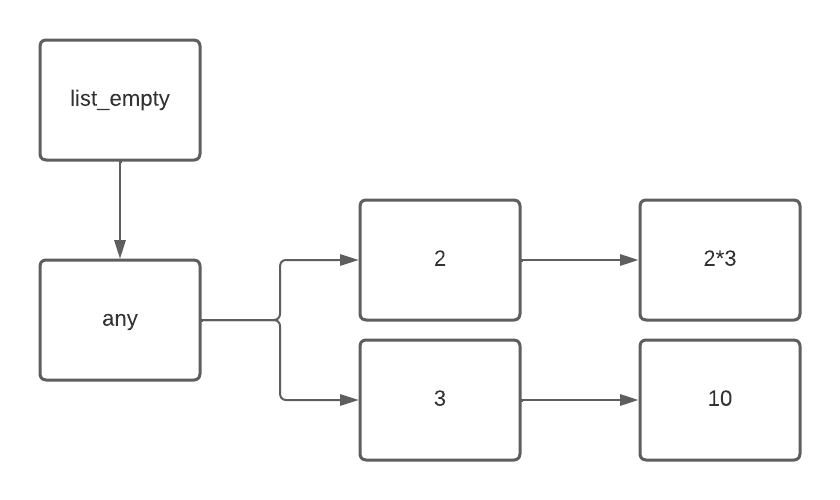
\includegraphics[width=0.5\textwidth]{Imagens/árvore.png}
    \caption{Árvore gerada}
\end{figure}

Em \textit{Python}:
\begin{minted}[xleftmargin=11pt]{python}
def example(arg0,arg1,arg2):
    if len(arg0) == 0:
        if arg2 == 2:
            a = arg1
            return 2*3
        elif arg2 == 3
            b = arg1
            return 10
        else raise ValueError
    else raise ValueError 
\end{minted}

\subsubsubsection{Estrutura de retorno de uma função}
\paragraph*{}
Consultar o apêndice \ref{appendix:estruturas_yacc} que fala sobre as estruturas.

\subsubsection{Funções}
\paragraph*{}
Na produção que contém a declaração de todas as funções, verifica-se, para cada uma, se já estava definida. Caso já esteja, adiciona-se um warning à variável do parser responsável por armazená-los. Caso não esteja, adiciona-se a função à variável do parser que contém todas as funções definidas e, também, à variável do parser que contém todas as funções definidas no bloco corrente.

\subsubsubsection{Estrutura de retorno}
\paragraph*{}
A estrutura contém apenas uma entrada com todas as chamadas de funções, de cada função.

\subsection{Produção Inicial}
\paragraph*{}
Na produção inicial, quanto a erros, apenas se verifica se as funções que foram chamadas estão presentes na variável do parser que contém todas as funções declaradas. Em caso negativo, é lançada uma exceção e o programa termina. De seguida, a tradução para \textit{Python} de todas as funções é junta numa só variável. Por fim, é efetuada uma pesquisa nessa variável que procura por chamadas de função e, para cada uma, acrescenta o prefixo "f\_" e o sufixo "\_". A estrutura de retorno da produção inicial é a string que contém o código todo traduzido.

\section{Compilador}
\paragraph*{}
O código para o compilador pode ler-se no apêndice \ref{appendix:fpyCompiler}.
O ficheiro \textit{fpyCompiler.py} do projeto é o programa referente ao nosso compilador. Pode-se executá-lo da seguinte forma:

\begin{minted}[xleftmargin=16pt]{bash}
    $ python3 fpyCompiler.py {nome_ficheiro}.py
\end{minted}

O programa lê todas as linhas do ficheiro de input e guarda numa string.
De seguida, utilizando o módulo re, encontramos nessa string todos os blocos FPY, e aplicamos uma função de substituição a cada bloco. Essa função de substituição tem acesso ao parser e ao lexer. Inicialmente, atualiza a linha inicial do lexer, atualiza a variável do parser que tem todas as funções declaradas no bloco atual para a lista vazia e, de seguida, aplica o parser ao texto a substituir. O resultado dessa operação substitui o bloco FPY capturado. De seguida, cria um ficheiro com o mesmo nome do ficheiro de input, mas com o sufixo "FPY" e escreve lá a string resultante. Por fim, ordena os warnings presentes na variável do parser por linha e imprime-os no terminal.


\chapter{Exemplos de utilização}
Neste capítulo damos um exemplo da aplicação do compilador a um ficheiro \textit{Python}.

\section*{Ficheiro original}
\inputminted[linenos,xleftmargin=16pt, breaklines=true, breakanywhere=true]{python}{Código/exemplo1.py}

\section*{Ficheiro originado}
\inputminted[linenos,xleftmargin=16pt, breaklines=true, breakanywhere=true]{python}{Código/exemplo1FPY.py}

\section*{Mensagens no \textit{standard output}}

\begin{minted}[xleftmargin=11pt]{bash}
56:5: <Warning> Redundant input in pattern matching for function 'mult_list_Num'
57:5: <Warning> Redundant input in pattern matching for function 'mult_list_Num'
95:5: <Warning> Redundant input in pattern matching for function 'mult'
98:1: <Warning> Function 'mult' is already defined
\end{minted}

\chapter{Conclusão} \label{concl}
\paragraph*{}
O projeto desenvolvido ajudou o grupo a aperfeiçoar os conhecimentos obtidos, durante o semestre, em Processamento de Linguagens. O tema escolhido permitiu-nos ainda relembrar o funcionamento de uma linguagem de programação funcional.

Tendo em conta o tema escolhido consideramos ainda que cumprimos com os requisitos propostos e ainda implementamos algumas funcionalidades extra, como a composição de funções, por exemplo. Como trabalho futuro, consideramos que podemos aumentar o nosso leque de tipo de dados permitidos e acrescentar mais funcionalidades típicas de linguagens funcionais.

\appendix

\chapter{Analisador Léxico}
\label{appendix:lexer}
\inputminted[linenos,xleftmargin=16pt, breaklines=true, breakanywhere=true]{Python}{Código/lexer.py}

\chapter{Analisadores Sintático e Semântico}
\label{appendix:parserGrammar}
\inputminted[linenos,xleftmargin=16pt, breaklines=true, breakanywhere=true]{Python}{Código/parserGrammar.py}

\chapter{Compilador FPY}
\label{appendix:fpyCompiler}
\inputminted[linenos,xleftmargin=16pt, breaklines=true, breakanywhere=true]{Python}{Código/fpyCompiler.py}

\chapter{Estruturas Yacc}
\label{appendix:estruturas_yacc}

\section{Statements}

Campos do statement:
\begin{itemize}
    \item \textbf{\textit{type}}: tipo da produção; 
    \item \textbf{\textit{python}}: tradução da produção para \textit{Python};
    \item \textbf{\textit{lexpos}}: posição do primeiro carácter da produção;
    \item \textbf{\textit{lineno}}: linha onde começa a produção;
    \item \textbf{\textit{lastpos}}: posição do ultimo carácter da produção;
    \item \textbf{\textit{func\_called}}: lista de funções que foram chamadas na produção. A lista contém tuplos no formato (número da linha,posição do primeiro carácter,nome da função);
    \item \textbf{\textit{vars}}: lista de variáveis utilizadas na produção. Esta lista contém tuplos no formato (número da linha,posição do primeiro carácter,identificador da variável).
    
\end{itemize} 

Tipos de dados possiveis num \textit{statement}:

\begin{itemize}
  \item \textbf{\textit{num}}: inteiros e floats;
  \item \textbf{\textit{boolean}}: booleanos;
  \item \textbf{\textit{any}}: identificadores de variáveis e chamadas de funções;
  \item \textbf{\textit{list\_(X)}}: lista de elementos do tipo X;
  \item \textbf{\textit{list\_}}: lista vazia ou lista com elementos do tipo \textit{any}.
\end{itemize}

\section{Case statement}

Campos do case statement:
\begin{itemize}
    \item \textbf{\textit{statement}}: tradução da sua atribuição para \textit{Python}; 
    \item \textbf{\textit{lexpos}}: posição do primeiro carácter da produção;
    \item \textbf{\textit{lineno}}: linha onde começa a produção;
    \item \textbf{\textit{lastpos}}: posição do ultimo carácter da produção;
    \item \textbf{\textit{func\_called}}: lista de funções que foram chamadas na sua atribuição;
    \item \textbf{\textit{input}}: Estrutura proveniente dos seus argumentos.
    
\end{itemize} 

\section{Função}

Campos da função:
\begin{itemize}
    \item \textbf{\textit{python}}: tradução da função para \textit{Python};
    \item \textbf{\textit{func\_name}}: nome da função;
    \item \textbf{\textit{lineno}}: linha onde começa a produção;
    \item \textbf{\textit{lexpos}}: posição do primeiro carácter da produção;
    \item \textbf{\textit{func\_called}}: lista de funções que foram chamadas nas suas atribuições.
    
\end{itemize} 

\chapter{Erros}
\label{appendix:erros}

\section{Formato}
\begin{minted}[xleftmargin=11pt]{bash}
numero_linha:numero_coluna: <tipo_erro> mensagem_erro
\end{minted}

\section{Possíveis Erros}
\subsection{Erros Léxicos}
\begin{itemize}
    \item Token reservado em \textit{Python}:\\ \mintinline{Python}{f"{linha}:{coluna}: <lexer error> Reserved python token '{caracter de erro}'"}
    \item Caracter ilegal:\\ \mintinline{Python}{f"{linha}:{coluna}: <lexer error> Illegal character '{caracter de erro}'"}
\end{itemize}
\subsection{Erros Sintáticos}
\begin{itemize}
  \item Token inesperado:\\ \mintinline{Python}{f"{linha}:{coluna}: <parse error> Unexpected token '{token}'"}
  \item Fim de input inesperado:\\ \mintinline{Python}{f"{linha}:{coluna}: <parse error> Unexpected end of input"}
\end{itemize}

\subsection{Erros Semânticos}
\begin{itemize}
\item Função não definida:  \\
  \mintinline{Python}{f"{linha}:{coluna}: <scope error> Function '{nome da função}' not in scope"}
  \item \mintinline[breaklines=true, breakanywhere=true]{Python}{f"{linha}:{Python}: <Error> Equations for function '{nome da função}' have different number of arguments"}
  \item Variável não definida: \\ \mintinline{Python}{f"{linha}:{coluna}: <scope error> Variable '{nome da variável}' not in scope"} 
  \item Variável já definida: \\ \mintinline{Python}{f"{linha}:{coluna}: <scope error> Variable '{nome da variável}' already in scope"}
 \item Incompatibilidade do tipo da expressão com o tipo esperado:\\ \mintinline[breaklines=true, breakanywhere=true]{Python}{f"{linha}:{coluna}: <type error> Couldn't match expected type '{tipo esperado}' with actual type '{tipo recebido}', in expression '{expressão}'"}
\end{itemize}

\chapter{Warning's}
\label{appendix:warnings}
\begin{itemize}
    \item Função já definida:\\ \mintinline{Python}{f"{linha}:{coluna}: <Warning> Function '{nome da função}' is already defined"}
    \item Input redundante:\\ \mintinline[breaklines=true]{Python}{f"{linha}:{coluna}: <Warning> Redundant input in pattern matching for function '{nome da função}'"}
\end{itemize}

\nocite{*}
\bibliographystyle{alpha}
\bibliography{bibliografia}

\end{document}
